
\section{Results}
\label{sec:results}

We now evaluate whether decomposing tool routing into semantic and compositional reasoning improves end-to-end performance compared to direct tool selection.

\subsection{Main Results}
\label{sec:main-results}

The decomposition improves F1 in every model--domain combination (20/20, average $\Delta$F1 = +0.32).
Table~\ref{tab:main-results} presents the full comparison.

\begin{table*}[t]
\centering
\small
\begin{tabular}{ll ccc ccc c}
\toprule
& & \multicolumn{3}{c}{\textbf{Baseline}} & \multicolumn{3}{c}{\textbf{TCR}} & \\
\cmidrule(lr){3-5} \cmidrule(lr){6-8}
\textbf{Model} & \textbf{Domain} & P & R & F1 & P & R & F1 & $\Delta$F1 \\
\midrule
Granite-8B & Kubernetes & 0.49 & 0.66 & 0.53 & 0.93 & 0.85 & 0.87 & +0.33 \\
 & Ansible & 0.27 & 0.51 & 0.34 & 0.83 & 0.83 & 0.81 & +0.47 \\
 & GitHub & 0.35 & 0.49 & 0.36 & 0.95 & 0.88 & 0.90 & +0.54 \\
 & CI/CD & 0.44 & 0.68 & 0.51 & 0.91 & 0.72 & 0.78 & +0.27 \\
 & Shopify & 0.63 & 0.85 & 0.69 & 0.93 & 0.90 & 0.90 & +0.22 \\
\midrule
Qwen3-14B & Kubernetes & 0.60 & 0.70 & 0.60 & 0.94 & 0.90 & 0.91 & +0.31 \\
 & Ansible & 0.36 & 0.52 & 0.41 & 0.73 & 0.69 & 0.71 & +0.30 \\
 & GitHub & 0.54 & 0.66 & 0.56 & 0.88 & 0.78 & 0.82 & +0.25 \\
 & CI/CD & 0.49 & 0.63 & 0.52 & 0.87 & 0.88 & 0.84 & +0.33 \\
 & Shopify & 0.83 & 0.81 & 0.79 & 0.96 & 0.90 & 0.92 & +0.13 \\
\midrule
GPT-OSS-20B & Kubernetes & 0.52 & 0.62 & 0.55 & 0.89 & 0.81 & 0.83 & +0.28 \\
 & Ansible & 0.25 & 0.46 & 0.32 & 0.79 & 0.74 & 0.76 & +0.44 \\
 & GitHub & 0.43 & 0.61 & 0.46 & 0.95 & 0.87 & 0.89 & +0.44 \\
 & CI/CD & 0.49 & 0.70 & 0.54 & 0.84 & 0.79 & 0.79 & +0.25 \\
 & Shopify & 0.36 & 0.53 & 0.39 & 0.92 & 0.89 & 0.90 & +0.51 \\
\midrule
Haiku-4.5 & Kubernetes & 0.49 & 0.81 & 0.58 & 0.94 & 0.90 & 0.91 & +0.33 \\
 & Ansible & 0.22 & 0.56 & 0.30 & 0.78 & 0.74 & 0.75 & +0.45 \\
 & GitHub & 0.53 & 0.76 & 0.59 & 0.88 & 0.91 & 0.88 & +0.29 \\
 & CI/CD & 0.48 & 0.75 & 0.55 & 0.71 & 0.83 & 0.73 & +0.18 \\
 & Shopify & 0.74 & 0.91 & 0.80 & 0.96 & 0.94 & 0.95 & +0.15 \\
\bottomrule
\end{tabular}
\caption{Baseline (direct tool selection) vs.\ TCR across all 20 model--domain combinations. TCR improves F1 in every case (avg.\ $\Delta$F1 = +0.32). All TCR outputs produce zero hallucinated tools.}
\label{tab:main-results}
\end{table*}

The improvement is consistent across models and domains.
A Wilcoxon signed-rank test over all 560 query-level comparisons confirms statistical significance ($p < 10^{-30}$; bootstrap 95\% CI: $[+0.27, +0.37]$).
The largest gains appear where baseline performance is weakest (Ansible: +0.30 to +0.47, GitHub: +0.25 to +0.54), suggesting that graph constraints are most valuable when unconstrained selection is hardest.

Among alternative strategies (Table~\ref{tab:strategy-comparison}), native function calling underperforms prompt-based selection across all models, and retrieval provides only modest improvements.
Neither enforces compositional validity.
The oracle (ground-truth types) achieves F1 = 1.000 across all domains, confirming that every benchmark workflow is representable as a graph path and that all remaining routing errors originate from entity type prediction.

\begin{table}[t]
\centering
\small
\begin{tabular}{l cccc}
\toprule
\textbf{Model} & \textbf{Base} & \textbf{Retr.} & \textbf{TCR} & \textbf{Oracle} \\
\midrule
Granite-8B  & 0.49 & 0.47 & \textbf{0.85} & 1.00 \\
Qwen3-14B   & 0.58 & 0.58 & \textbf{0.84} & 1.00 \\
GPT-OSS-20B & 0.45 & 0.53 & \textbf{0.83} & 1.00 \\
Haiku-4.5   & 0.56 & 0.57 & \textbf{0.84} & 1.00 \\
\bottomrule
\end{tabular}
\caption{Average F1 across domains by strategy. TCR consistently outperforms both prompt-based and retrieval-based selection. Oracle F1 = 1.000 confirms complete graph coverage.}
\label{tab:strategy-comparison}
\end{table}

\subsection{Structural Validity}
\label{sec:structural-validity}

As guaranteed by Proposition~1 (Section~\ref{sec:tcr}), TCR produces zero hallucinated tools across all model--domain combinations.
The baseline produces hallucinated tools in most runs (1--16 per model across domains).
This is not an empirical observation but a structural property: graph search traverses only registered edges.

\subsection{Recall Decomposition}
\label{sec:recall-decomposition}

Table~\ref{tab:recall-decomposition} presents the decomposition from Eq.~\ref{eq:recall-decomposition}, separating routing performance into entity type prediction quality and graph recoverability.

\begin{table}[t]
\centering
\small
\begin{tabular}{l ccc}
\toprule
\textbf{Model} & $P_c$ & $R_c$ & $R_{\text{wrong}}$ \\
\midrule
Granite-8B  & 0.54 & 0.95 & 0.33 \\
Qwen3-14B   & 0.60 & 0.96 & 0.24 \\
GPT-OSS-20B & 0.62 & 0.92 & 0.29 \\
Haiku-4.5   & 0.65 & 0.95 & 0.30 \\
\bottomrule
\end{tabular}
\caption{Recall decomposition (averaged across domains). $P_c$ = exact match type accuracy. $R_c$ = recall when types are correct. $R_{\text{wrong}}$ = recall when types are incorrect. High $R_c$ ($>$0.92) confirms the graph reliably recovers correct workflows; non-zero $R_{\text{wrong}}$ shows graceful degradation.}
\label{tab:recall-decomposition}
\end{table}

When entity types are correct, recall averages 0.95 across all models, confirming that the graph reliably recovers the expected tool chains.
Performance does not collapse when prediction is wrong: $R_{\text{wrong}}$ averages 0.29, meaning incorrect types still recover part of the correct workflow.
This graceful degradation arises because neighboring entity types often share downstream graph paths.

Figure~\ref{fig:type-vs-f1} provides direct evidence for the relationship between type prediction and routing: exact-match accuracy correlates strongly with F1 (Pearson $r = 0.71$, $p < 0.001$, $R^2 = 0.50$).

\begin{figure}[t]
\centering
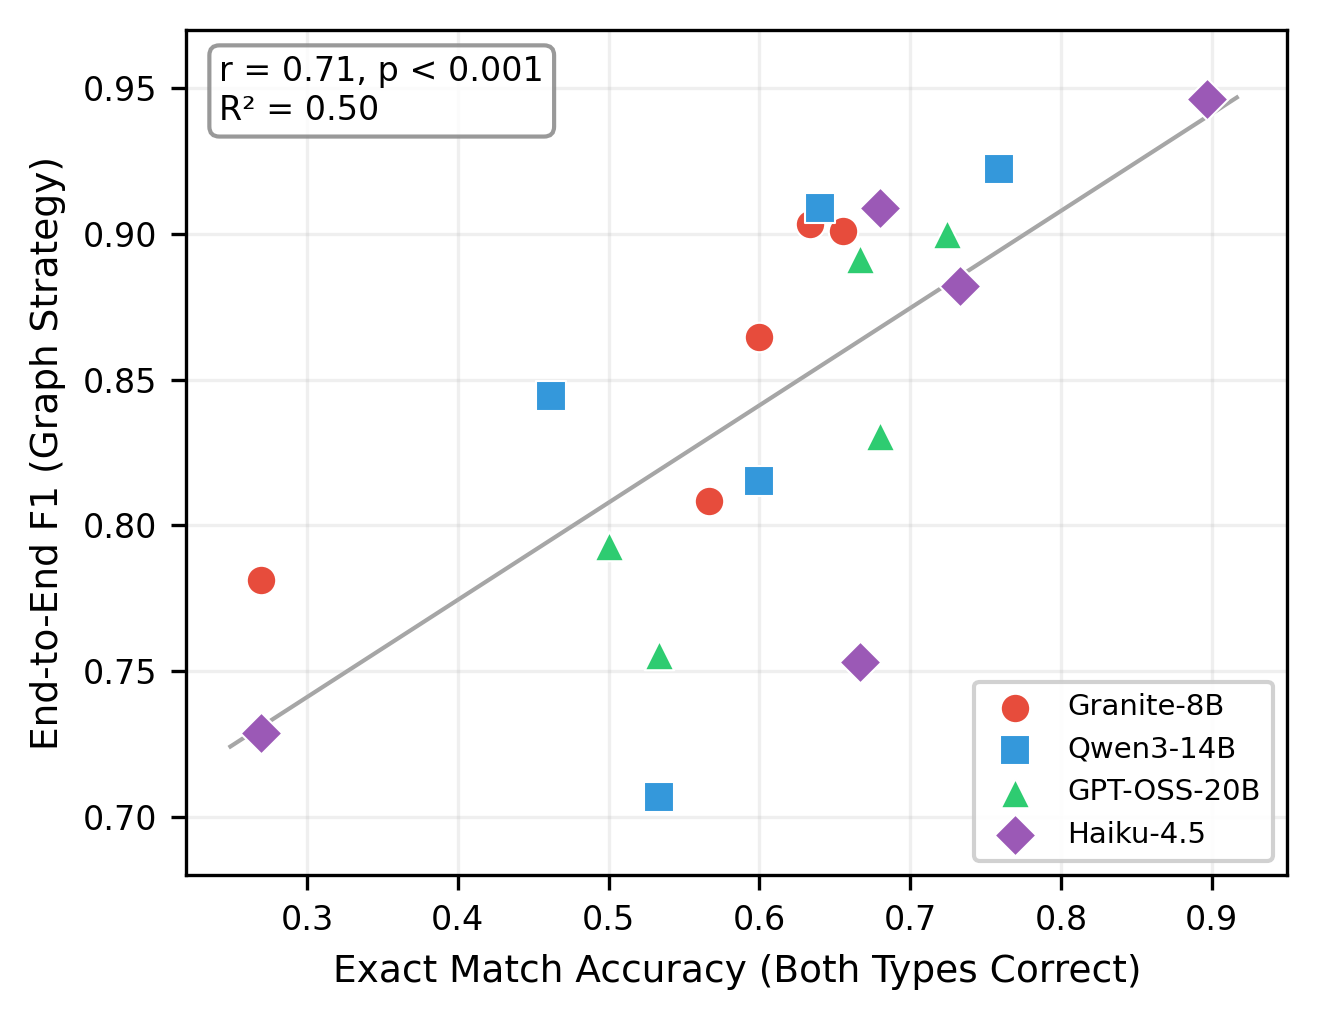
\includegraphics[width=\columnwidth]{figures/scatter_type_prediction_vs_f1.pdf}
\caption{Entity type prediction accuracy vs.\ end-to-end F1 across all 20 model--domain combinations (Pearson $r = 0.71$, $p < 0.001$). Type prediction quality is a strong predictor of routing performance.}
\label{fig:type-vs-f1}
\end{figure}


\subsection{Entity Pruning}
\label{sec:entity-pruning}

The median entity pruning across all domains is 75\%: for a typical query, three-quarters of source candidates are structurally eliminated after target prediction.

CI/CD provides the strongest evidence that graph topology, not label-space reduction, drives TCR's advantage.
With 51 types for 54 tools (near-parity), the type space offers almost no label reduction, yet entity pruning averages 87\%.
Even the hardest CI/CD query constrains the source to at most 12 of 51 candidates.

\subsection{Type Prediction Accuracy}
\label{sec:type-prediction}

\begin{table}[t]
\centering
\small
\begin{tabular}{l ccc}
\toprule
\textbf{Category} & \textbf{Source} & \textbf{Target} & \textbf{Both} \\
\midrule
Clean & 0.82 & 0.95 & 0.81 \\
Multi-hop & 0.65 & 0.96 & 0.64 \\
Noisy & 0.57 & 0.84 & 0.54 \\
Synonym & 0.71 & 0.61 & 0.50 \\
Ambiguous & 0.58 & 0.32 & 0.25 \\
Multi-path & 0.53 & 0.69 & 0.38 \\
\midrule
Overall & 0.70 & 0.80 & 0.61 \\
\bottomrule
\end{tabular}
\caption{Type prediction accuracy by query category (averaged across models and domains). Source prediction (0.70) is harder than target (0.80), consistent with users describing desired outcomes more clearly than starting points.}
\label{tab:type-prediction}
\end{table}

Table~\ref{tab:type-prediction} reports type prediction accuracy by query category.
Target prediction (0.80) is easier than source prediction (0.70), consistent with the intuition that users describe desired \emph{outcomes} more clearly than \emph{starting points}.
Clean queries achieve 81\% exact match; ambiguous queries are hardest (25\%), since the target type is genuinely uncertain.
Since the recall decomposition confirms that routing performance tracks type prediction quality, improving entity type prediction is the primary lever for improving end-to-end performance.


\subsection{Scaling to Production Tool Ecosystems}
\label{sec:production-eval}

The preceding results validate the decomposition on benchmark domains with 54--170 tools.
A natural question is whether the formulation remains effective at significantly larger scale, and whether the composition graph can be constructed automatically rather than by hand.
We test both by evaluating on the official Ansible Automation Platform MCP Server, a production system with 1,060 tool operations and 79 entity types derived automatically from OpenAPI specifications.
At this scale, the 1,060 tool schemas require $\sim$64,000 tokens---exceeding the entire 32K context window of models like Qwen3-14B, making function calling physically impossible without truncation.
Even for models with larger context windows, the text baseline consumes $\sim$18,000 prompt tokens per query.
Under the decomposed formulation, the LLM reasons over 79 entity type names rather than 1,060 tool definitions, reducing prompt tokens to $\sim$300 (99.5\% reduction).

\begin{table}[t]
\centering
\small
\begin{tabular}{l c c c c}
\toprule
\textbf{Model} & \textbf{Strategy} & \textbf{F1} & \textbf{Prec.} & \textbf{Rec.} \\
\midrule
\multirow{2}{*}{Granite 8B}
    & Baseline & 0.61 & 0.58 & 0.69 \\
    & TCR      & \textbf{0.74} & \textbf{0.74} & \textbf{0.73} \\
\midrule
\multirow{2}{*}{Qwen3-14B}
    & Baseline & 0.66 & 0.63 & 0.73 \\
    & TCR      & \textbf{0.80} & \textbf{0.81} & \textbf{0.80} \\
\midrule
\multirow{2}{*}{Haiku 4.5}
    & Baseline & 0.58 & 0.50 & 0.74 \\
    & TCR      & \textbf{0.91} & \textbf{0.91} & \textbf{0.91} \\
\bottomrule
\end{tabular}
\caption{Results on the AAP MCP Server (1,060 tools, 79 entity types, 47 queries). TCR improves F1 for all models with zero hallucinations. The oracle achieves F1 = 1.000, confirming complete graph coverage. When entity types are correct, $R_c$ = 1.000 for all three models.}
\label{tab:aap-results}
\end{table}

Table~\ref{tab:aap-results} presents results on 47 operator workflow queries.
TCR improves F1 for all three models ($\Delta$F1: +0.13 to +0.33) with zero hallucinated tool invocations.
The oracle achieves F1 = 1.000, confirming complete graph coverage.
The recall decomposition fits exactly: when entity types are correct, $R_c$ = 1.000 for all three models.

Type prediction accuracy ranges from 72\% (Granite 8B) to 91\% (Haiku 4.5) exact match over 79 automatically derived types, comparable to or exceeding the five benchmark domains.
A notable model ranking inversion occurs: under the baseline, Qwen3-14B achieves the highest F1 (0.66) and Haiku the lowest (0.58); under TCR, this reverses (Haiku 0.91, Granite 0.74).
The two formulations reward different capabilities---direct selection rewards scanning long tool lists, while the decomposition rewards semantic understanding of domain entities.

These results confirm that the decomposition scales beyond benchmark-sized domains: at 1,060 tools, separating semantic reasoning from compositional reasoning remains effective, and the composition graph can be derived automatically from existing API specifications.
